\documentclass[11pt]{article}

\usepackage[T1]{fontenc}
\usepackage{lmodern}
\usepackage[a4paper,margin=2.5cm]{geometry}
\usepackage{microtype}
\usepackage{amsmath}
\usepackage{booktabs}
\usepackage{tabularx}
\usepackage{xcolor}
\usepackage{tikz}
\usepackage[round,authoryear]{natbib}
\usepackage[hidelinks]{hyperref}

\newcommand{\code}[1]{\texttt{#1}}
% File and script names: break at underscores, slashes and dots.
\makeatletter\g@addto@macro\UrlBreaks{\do\_}\makeatother

\title{Confidently Constant: Token Probabilities Reveal Input-Insensitive Decisions\\
in an LLM-Agent Simulation of Democracy}
% The author line is the owner's to fill before submission.
\author{[Author name]\\[2pt]\small [Affiliation, e-mail]}
\date{Draft, \today}

\begin{document}
\maketitle

\begin{abstract}
Simulations that hand their agents' decisions to a large language model (LLM) are usually
checked on their outputs: does the simulated society behave plausibly? We report a case where
the aggregates raised no alarm while three decisions barely depended on their inputs. Polity is
a simulated democracy in which many decisions of citizens, parties and an elected officeholder
are delegated to an LLM (Qwen3-8B in its 4-bit AWQ build, served by vLLM), as closed codes in
schema-constrained JSON. We built an instrument that reads, in a completion made exactly as
production makes it, the probability the model gives a code at the token where it writes it,
and that raises an error on the misalignments it can detect. Checked first on a decision with a computable rule (16 voters, mean probability 0.997
against 0.049), it was then pointed at three decisions whose inputs we swept between extremes at
temperature~0. An officeholder's probability of conceding to protest stayed between 0.999999 and
1.000000 over nine situations, a party's probability of joining a coalition between 0.965 and
0.999 over five, and a citizen's probability of waiting for the next election at or above
0.9756 for all seventeen citizens, from the most satisfied to the angriest. The citizen's
decision was invisible in the simulation's aggregates by construction, and its prompt omitted
the criterion the simulation scored it against. Calibrating the two other prompts restored
little. The coalition decision also stayed flat on a 4B base/instruct pair and on one other
model family (a second family's reading proved unusable), while the officeholder's decision did
not collapse on the 4B model. We describe the instrument, its limits, and the practice it led to:
a table of the decision types a scientific claim may rest on, and probing a decision before
running an experiment on it, which stopped one experiment.
\end{abstract}

% ---------------------------------------------------------------------------------------
\section{Introduction}

LLM-driven agents are now a common way to simulate people: in sandboxes of believable
characters \citep{park2023generative}, as ``silicon samples'' of survey respondents
\citep{argyle2023outofone}, in replications of human-subject studies \citep{aher2023turing}, and
in agent-based models of social systems \citep{gao2024abmsurvey}. A recurring worry is that such
agents are less varied than the people they stand for
\citep{bisbee2024synthetic,wang2025flatten,anthis2025position}.

Most of that evidence compares a model's answers with a human reference. A simulation whose
agents feed each other has a different, more basic question to answer first: does each LLM
decision depend on the inputs it is given? A simulated society can look plausible in aggregate
while individual decisions ignore their inputs. Aggregates can even match what a working
decision would produce, as we show in Section~\ref{sec:aggregates}.

This paper is a case study of that question in Polity, a simulated democracy. Its contribution is
fourfold.
\begin{enumerate}
  \item \textbf{An instrument} that reads the probability of each closed code from completions
    made with the production prompts and schemas: schema-constrained JSON, sometimes preceded by
    a reasoning block, several decisions per call. It aligns each decision field to the token
    that wrote it, raises an error on the misalignments it can detect, and has known silent cases
    that we state (Section~\ref{sec:instrument}).
  \item \textbf{Three input sweeps} on which a decision's probability barely moved between
    situations that should have called for opposite answers (Section~\ref{sec:sweeps}). Drawing
    each decision from its own probability instead of taking the top answer would change
    almost nothing: the model was confidently constant.
  \item \textbf{A diagnosis}, partial. One prompt omitted the criterion the simulation scored
    the decision against. Calibrating the other two prompts restored little. The coalition
    decision stayed flat on a 4B base/instruct pair and on one other model family
    (Section~\ref{sec:diagnosis}).
  \item \textbf{A practice}: a table of decision types fit for inference, and probing a
    decision before an experiment relies on it (Section~\ref{sec:practice}).
\end{enumerate}
The probes are small, mostly on one model, and mostly single runs at temperature~0.
Section~\ref{sec:limits} states what they do not show.

% ---------------------------------------------------------------------------------------
\section{Related work}

\paragraph{LLMs as simulated people.} Generative agents \citep{park2023generative}, silicon
samples \citep{argyle2023outofone} and simulated subject pools \citep{aher2023turing} made LLM-driven social simulation practical, and
surveys and position papers chart its promise and its open challenges, among them outputs that
are generic or stereotyped \citep{gao2024abmsurvey,anthis2025position}. Evidence of reduced
variety has accumulated at the level of answer distributions. Models' opinions diverge from those
of human groups \citep{santurkar2023whose}. Synthetic survey answers vary less than human ones
and shift with prompt wording \citep{bisbee2024synthetic}. Survey answers are dominated by
ordering and labelling biases, and trend towards uniform once those are adjusted for
\citep{dominguezolmedo2024questioning}. Models fail to reproduce human response biases
\citep{tjuatja2024responsebiases}, and identity-conditioned answers flatten groups
\citep{wang2025flatten}. Preference tuning reduces output diversity \citep{kirk2024rlhf}. These
studies compare a model's answers with a human reference. Ours has none: the question is whether
a decision moves with its own inputs.

\paragraph{Probabilities rather than samples.} Token probabilities are the usual way to score
closed answers and to study calibration \citep{kadavath2022know}. Their pitfalls are known:
selection bias towards particular option labels \citep{zheng2024selectors}, sensitivity to
formatting \citep{sclar2024formatting}, and first-token probabilities that disagree with the
answer the model actually writes \citep{wang2024myanswerisc}. Our instrument avoids the
first-token shortcut. It reads the probability at the token where the code is written, inside
the model's own constrained output and after any reasoning, and refuses when it cannot locate
that token.

% ---------------------------------------------------------------------------------------
\section{Setting}
\label{sec:setting}

\paragraph{Polity.} Polity simulates citizens (100 or 500 in the runs cited here), parties and an
elected officeholder over repeated elections. Nine of its decisions can be delegated to the LLM.
Each is a chat completion whose answer is JSON under a schema, from which the simulation reads
one closed code per agent. Several agents' decisions are often asked in one call, as a list. This
paper concerns four of the nine decisions:
\begin{itemize}
  \item \textbf{\code{vote\_cast}}: a voter's ballot, including whether to cast a blank vote;
  \item \textbf{\code{representative\_response}}: the officeholder's stance when the street
    mobilises: 1~concession, 2~defiance, 3~silence or 4~counter-mobilisation;
  \item \textbf{\code{coalition\_decision}}: a party offered a place in a coalition: 1~join or
    2~leave;
  \item \textbf{\code{pressure\_action}}: a discontented citizen between elections. In the shipped
    configuration the menu was closed to 0~do nothing and 4~wait for the election.
\end{itemize}

\paragraph{Serving.} The production model is Qwen3-8B \citep{qwen2025qwen3} in its official
4-bit AWQ build (\code{Qwen/Qwen3-8B-AWQ}, pinned revision, \code{awq\_marlin} kernels), served by
vLLM \citep{kwon2023vllm} on one 16\,GB consumer GPU, with the \code{qwen3} reasoning parser and
xgrammar structured outputs. The check against a known rule, the sweeps and the calibrations
(Sections~\ref{sec:instrument} to~\ref{sec:calibration}) ran on vLLM 0.28.0. The case bank's Qwen
control (Section~\ref{sec:diagnosis}) ran on vLLM 0.30.0, and the threshold probe
(Section~\ref{sec:practice}) on 0.31.0. The client used
temperature~0, seed~42 and the top~10 log-probabilities per token. The model's thinking mode was
on for the vote and off for the three other decisions. Section~\ref{sec:diagnosis} names the
other models and servers used.

% ---------------------------------------------------------------------------------------
\section{Reading a decision, not an answer}
\label{sec:instrument}

A sampled answer tells you what the model said once, not how close it came to saying something
else. For a closed code there is a better reading: the probability the model assigns to each code
at the token where it writes it. vLLM returns the top log-probabilities for every generated token,
so if the answer contains \code{"act": 4}, one can read $P(4)$ against $P(0)$ at the token where the
\code{4} was written.

\paragraph{Locating the token.} On production prompts this is not trivial, for three reasons.
\begin{itemize}
  \item \textbf{Hidden reasoning:} the server's reasoning parser removes the
    \code{<think>} block from the answer's text but not from its token stream. The instrument
    rebuilds the raw text by concatenating the tokens, finds the answer inside it (the rightmost
    match), and works in raw character offsets.
  \item \textbf{Several decisions per call:} it finds each occurrence of the decision field in
    document order, pairs them with the parsed list of decisions, and checks that each has its
    identifier.
  \item \textbf{The covering token:} for each decision it takes the token whose character span
    covers the field's value.
\end{itemize}

\paragraph{When it refuses.} It raises an error, never returning a partial reading, when the
answer is not found in the raw stream, when a value is not a scalar, when the occurrences and the
decisions differ in number, when a decision lacks its identifier, or when no token covers the
value.

\paragraph{Readers.} Two readers turn the token's top-10 alternatives into a number:
\begin{itemize}
  \item \textbf{normalised} over two named codes, $P(a)/(P(a)+P(b))$, used for the blank vote and
    the citizen's action;
  \item \textbf{raw}, $\exp$ of one code's log-probability, used for the officeholder's stance
    and the coalition decision. These are not renormalised over the other codes.
\end{itemize}

\paragraph{Silent cases.} Both readers return a value rather than an error when a code falls
outside the top~10: the normalised reader returns 0.5 if neither code is present, and the raw
reader returns 0.0. Multi-digit codes that share a leading digit defeated the alignment silently.
Every code sat on an identical token, and one probe of a reaction decision read exactly 0.500000
at every point, until an offset into the value was added. A flat reading near 0.5 or 0.0 is
therefore a reason to check, not a result.

\paragraph{A check against a known rule.} One decision has a computable answer: whether a voter
casts a blank ballot follows a rule of the simulation. We selected 16 voters from a pool of 200,
the first 8 for whom the rule says blank and the first 8 for whom it does not. We asked the
production vote prompt with reasoning on, in calls of three voters as in production. All 16
readings aligned, and the readings put all 16 on the right side of 0.5. The mean
$P(\text{blank})$ was 0.9969 for the first group and 0.0494 for the second, a separation of
$+0.948$. This shows that the instrument reads the right token and that the probability tracks
the rule on clear cases. It is not a calibration curve. None of the 16 voters sat near their own
threshold. The version of this check in a later case bank, with a different voter pool and
nomination rule, aligned 13 of 16 readings on this model with the request settings of that
time. With the vote grammar that production has used since 2026-09-16, it aligned 16 of 16, at a
lower separation ($+0.652$ against $+0.942$).

% ---------------------------------------------------------------------------------------
\section{Three flat lines}
\label{sec:sweeps}

Each probe used the production prompt builders and schemas unchanged. It moved the inputs from
a situation calling for one answer to one calling for the other, and read the probability at
each point. Two of the three moved several inputs together, which is enough to test whether the
decision moves at all, but not which input it ignores. Table~\ref{tab:sweeps} summarises them,
and Figure~\ref{fig:sweeps} plots two.

\begin{table}[t]
\centering\small
\begin{tabularx}{\linewidth}{@{}lXcl@{}}
\toprule
Decision & Inputs moved, from one extreme to the other & Points & Reading \\
\midrule
\code{representative\_response} &
  Legitimacy 0.95$\to$0.05, mandate deviation 0.0$\to$0.8, street 0.0$\to$3.0, time to the
  election 20$\to$2, together; one officeholder per call &
  9 & $P(\text{concede})$: 0.999999--1.000000 \\
\code{coalition\_decision} &
  Platform distance 0$\to$4.47 (20 issues) and seats missing 25$\to$0, together; five parties per
  call &
  5 & $P(\text{join})$: 0.964855--0.999374 \\
\code{pressure\_action} &
  The citizen's gap to the officeholder, 0.02$\to$2.20; seventeen citizens in one call &
  17 & $P(\text{wait})$: $\geq 0.9756$ \\
\bottomrule
\end{tabularx}
\caption{The three input sweeps on Qwen3-8B-AWQ, temperature 0. The first two readings are raw,
the third normalised over its two codes (Section~\ref{sec:instrument}).}
\label{tab:sweeps}
\end{table}

\paragraph{The officeholder's response.} Over nine points, from high legitimacy with nobody in the
street to low legitimacy with a large crowd, $P(\text{stance}=1)$, conceding, read between 0.999999
and 1.000000. Its full spread was 0.000001.\footnote{The calibration study of
Section~\ref{sec:calibration} describes this baseline as 0.999996 to 1.000000; the per-point table
gives the range above.}

\paragraph{The coalition offer.} Five parties along a diagonal: the first identical to the
initiator, whose coalition was 25 seats short, the last maximally distant on all 20 issues, with
no seats missing. $P(\text{join})$ read 0.999374, 0.992539, 0.964855, 0.999015 and 0.996777. The two
ends differ by $-0.0026$, and the low point is in the middle, not at the end.

\paragraph{The citizen's action.} Seventeen citizens with gaps to the officeholder from 0.02 to
2.20, all in one call. The probability of waiting for the election averaged 0.9961 below a gap of
0.5 and 0.9999 above it, a separation of $+0.0039$. Every citizen but the most satisfied, at
0.9756, read 0.9966 or more. Asked alone, the two extreme citizens read 0.999992 and 1.000000.

\paragraph{Confident, not marginal.} These are not weak preferences that a different draw would
flip. If each citizen's decision were drawn from its own probability instead of taking the top
answer, the expected number of decisions that change, $\sum_i \min(p_i, 1-p_i)$, would be 0.03 of
17. In the four configurations where it was computed, three of them on the 4B models of
Section~\ref{sec:diagnosis}, it was at most 0.96 of 17.

\begin{figure}[t]
\centering
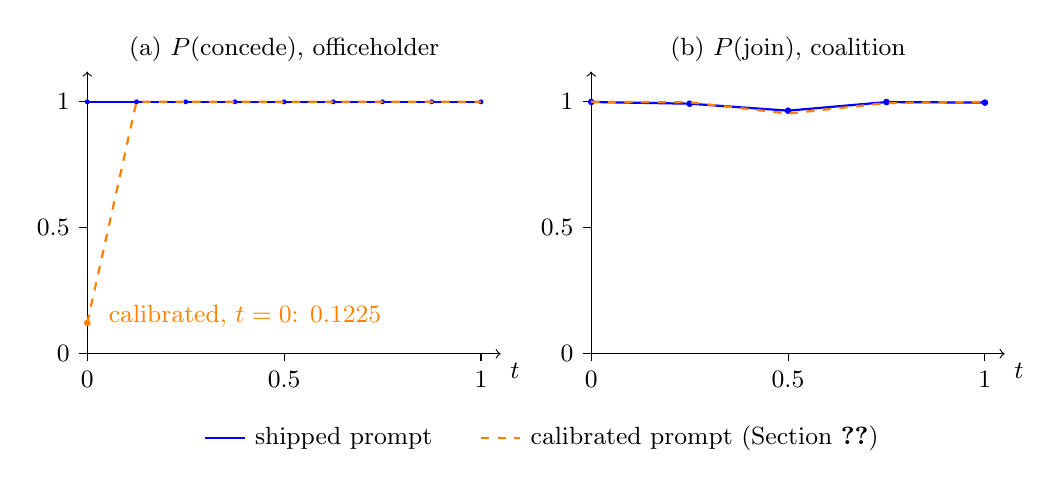
\begin{tikzpicture}[x=5cm,y=3.2cm,font=\small]
  % Panel (a): the officeholder's response
  \begin{scope}
    \draw[->] (0,0) -- (1.05,0) node[below right] {$t$};
    \draw[->] (0,0) -- (0,1.12);
    \foreach \y in {0,0.5,1} \draw (0,\y) -- (-0.02,\y) node[left] {\y};
    \foreach \x in {0,0.5,1} \draw (\x,0) -- (\x,-0.03) node[below] {\x};
    \node[above] at (0.5,1.12) {(a) $P(\text{concede})$, officeholder};
    \draw[thick,blue] (0,1) -- (0.125,0.999999) -- (0.25,1) -- (0.375,1) -- (0.5,1) -- (0.625,1)
      -- (0.75,1) -- (0.875,1) -- (1,0.999999);
    \foreach \x in {0,0.125,...,1} \fill[blue] (\x,1) circle (0.9pt);
    \draw[thick,orange,dashed] (0,0.122522) -- (0.125,0.999999) -- (0.25,1) -- (1,1);
    \fill[orange] (0,0.122522) circle (1.2pt);
    \node[right,orange] at (0.03,0.15) {calibrated, $t=0$: 0.1225};
  \end{scope}
  % Panel (b): the coalition offer
  \begin{scope}[xshift=6.4cm]
    \draw[->] (0,0) -- (1.05,0) node[below right] {$t$};
    \draw[->] (0,0) -- (0,1.12);
    \foreach \y in {0,0.5,1} \draw (0,\y) -- (-0.02,\y) node[left] {\y};
    \foreach \x in {0,0.5,1} \draw (\x,0) -- (\x,-0.03) node[below] {\x};
    \node[above] at (0.5,1.12) {(b) $P(\text{join})$, coalition};
    \draw[thick,blue] (0,0.999374) -- (0.25,0.992539) -- (0.5,0.964855) -- (0.75,0.999015)
      -- (1,0.996777);
    \foreach \x/\y in {0/0.999374,0.25/0.992539,0.5/0.964855,0.75/0.999015,1/0.996777}
      \fill[blue] (\x,\y) circle (1.2pt);
    \draw[thick,orange,dashed] (0,0.999888) -- (0.25,0.998012) -- (0.5,0.953275) -- (0.75,0.995318)
      -- (1,0.999497);
  \end{scope}
  % Legend
  \begin{scope}[yshift=-0.75cm]
    \draw[thick,blue] (0.3,-0.1) -- (0.4,-0.1) node[right,black] {shipped prompt};
    \draw[thick,orange,dashed] (1.0,-0.1) -- (1.1,-0.1) node[right,black] {calibrated prompt
      (Section~\ref{sec:calibration})};
  \end{scope}
\end{tikzpicture}
\caption{Two of the sweeps, from the situation calling for one answer ($t=0$) to the one calling
for the other ($t=1$), on the full probability scale. (a) The officeholder: conceding at
legitimacy 0.95 with an empty street ($t=0$) as at legitimacy 0.05 with a crowd ($t=1$). (b) A
party offered a coalition: joining when identical and needed ($t=0$) as when maximally distant and
not needed ($t=1$).}
\label{fig:sweeps}
\end{figure}

% ---------------------------------------------------------------------------------------
\section{Why the aggregates did not show it}
\label{sec:aggregates}

For the citizen's action, the shipped menu offered two codes, neither of which counts as
mobilising. A mobilisation rate of zero is therefore what that menu predicts whether the decision
works or not. A constant answer and a working one produce the same aggregate, and only a
per-citizen reading can tell them apart.

The two other decisions do show in the totals, but a total cannot say whether a decision followed
its inputs. In ten runs of 100 citizens, coalition offers were accepted 152 times in 160. After a
partial fix of the officeholder's prompt, two runs of 500 citizens still had the officeholder
conceding in 33 of 33 model answers, and in 25 of 32. That could describe a cooperative
society. Whether real inputs ever called for another answer was not established. So these counts
are consistent with the flat readings but do not prove them; only varying the inputs does.

% ---------------------------------------------------------------------------------------
\section{What the flat lines were made of}
\label{sec:diagnosis}

\subsection{A criterion the prompt never sent}

The simulation scores the citizen's action by comparing the citizen's gap with the citizen's own
tolerance threshold. The prompt sent the gap, and never sent the threshold. The model was asked
whether a citizen was discontented enough to act, given a number with no scale. The blank-vote
prompt, which tracked its rule, states its quantity, its threshold and its rule.

Supplying the threshold was not enough on its own (Table~\ref{tab:pressure}). Added as data to
the 17-citizen call, it barely moved the readings. A control prompt that stated the rule through
to the action separated the two extreme citizens almost perfectly when each was asked alone
(0.007346 against 1.000000, $+0.9927$), but read flat ($+0.0001$) for the same 17 citizens in one
call. Batches were unstable in both directions. With citizens in alternating order, agreement with
the rule fell to 0 of 12 at one size: the model was completing the alternating pattern instead
of reading the values. With the order permuted once, the same sizes scored 2/2, 8/8, 12/12,
17/17 and 24/25. With the order randomised, agreement swung between 0\% and 100\% from one
trial to the next at the same size. Accuracy depended on the batch's composition and order rather
than on its size.

Note that batching does not explain the original flat line. The shipped prompt was flat when
asked about one citizen alone too ($+0.000008$, Section~\ref{sec:sweeps}).

\begin{table}[t]
\centering\small
\begin{tabular}{@{}lrrc@{}}
\toprule
Prompt (17 citizens, one call) & mean $P(\text{act}=4)$ & separation & agrees with rule \\
\midrule
A\quad shipped & 0.9982 & $+0.0038$ & 9/17 \\
B\quad A + the threshold, as data & 0.9781 & $+0.0462$ & 9/17 \\
C\quad B + a rule from gap to acceptability & 0.0035 & $+0.0004$ & 8/17 \\
D\quad B + the rule through to the action & 0.9999 & $+0.0001$ & 9/17 \\
\midrule
D, the two extremes asked one at a time & 0.007346 / 1.000000 & $+0.9927$ & 2/2 \\
\bottomrule
\end{tabular}
\caption{The citizen's action. A constant answer agrees with the rule on 8 or 9 of these 17
citizens. Prompt A is the shipped prompt, run again within this study ($+0.0038$ here, $+0.0039$
in Section~\ref{sec:sweeps}). Prompts C and D state the rule, which the shipped simulation does not do on purpose: a
model executing a rule written into its prompt is a slow copy of the rule. They are controls of
the model's capability, not fixes.}
\label{tab:pressure}
\end{table}

\paragraph{What shipped.} The fix sends the threshold as data, with no rule, and asks one citizen
per call. Before shipping it, five prompt variants were tested on unambiguous citizens of a
generated population at batch sizes of 1, 5 and 25, three trials each. All failed at 5 and 25,
near the agreement a constant answer would get. At size~1, the four variants tested there agreed
in every trial. A later correction found that those trials had drawn only citizens on one side of the threshold, where a
constant answer also scores 100\%. Live, end to end, the shipped decision agreed with the rule
on 12 of 12 citizens, six on each side, where a constant answer gets 6. On a frozen bank of 24
cases, 12 on each side, it agreed on 15, where a constant gets 12. The decision is no longer
constant, and it is not validated.

\subsection{Calibrating the other two}
\label{sec:calibration}

The officeholder's prompt gave units but no scale. Stating two bounds that were always true, that
the mandate deviation lies in $[0,1]$ and the street's realistic ceiling, moved only one point.
At legitimacy 0.95 with nothing in the street, $P(\text{concede})$ fell to 0.1225, and the model
chose silence. Every other point stayed at 0.999999 or 1.000000 (Figure~\ref{fig:sweeps}a). The
response now separates ``no problem at all'' from ``any problem''. It does not grade the problem.

The coalition prompt gave a platform distance with no reference. One sentence giving the mean
distance among the seated parties changed nothing measurable: the ends differed by $-0.0004$ and
every reading stayed at or above 0.953 (Figure~\ref{fig:sweeps}b). Joining may be a policy the model
converges on for institutional reasons, and not obviously a defect. What fails is the
simulation's own contract that platform distance should matter.

\subsection{Is it one model? Is it instruction tuning?}

\paragraph{A 4B pair.} Qwen3-4B and Qwen3-4B-Base, both in bf16, both served by the same vLLM
0.28.0 build with identical flags, differ in post-training. The pair answers the question only if
the collapse reproduces on the 4B instruct model, so we checked that first, with the
uncalibrated prompts.
\begin{itemize}
  \item \textbf{Coalition:} flat on the 4B instruct model ($P \approx 1.0$, spread 0.00043).
  \item \textbf{Citizen's action:} flat too, but at the opposite constant, $P(\text{act}=4) \approx 0$.
  \item \textbf{Officeholder:} \emph{not} flat. At the no-problem pole the 4B model chose silence
    ($P(\text{concede}) = 0.000000$), and at every pressured point conceded (1.000000).
\end{itemize}
So instruction tuning alone does not produce the officeholder's flatness. Between the 8B and
4B models, parameter count, post-training recipe and quantisation all differ, so the difference
cannot be attributed to any one of them.

Table~\ref{tab:basevsinstruct} compares the two arms on the two decisions that reproduced. The
bar, $|\text{separation}| \geq 0.10$ with the correct sign where the instruct model showed at most
0.03, was written before the base arm ran, restating an earlier pre-registered bar after the
instruct run. Neither arm cleared it on the primary, batched statistic, on either decision; the
base model's solo control crossed it ($+0.124$). The base
model's readings moved more with the citizen's gap in both geometries. But the instruct model
also correlated significantly in the second geometry, and the emitted decision was the same
for every citizen in all four arm-by-geometry cells. A base model completing a chat-formatted
instruction prompt is also not doing the same task as the instruct model.

\begin{table}[t]
\centering\small
\begin{tabular}{@{}llcc@{}}
\toprule
Decision & Statistic & 4B instruct & 4B base \\
\midrule
\code{pressure\_action}, geometry A & separation (batch of 17) & $-0.029$ & $+0.089$ \\
 & Pearson $r$ with the gap & $-0.117$ & $+0.378$ \\
 & separation, extremes alone & $+0.093$ & $+0.124$ \\
\code{pressure\_action}, geometry B & separation & $+0.017$ & $+0.073$ \\
 & Pearson $r$ ($p$) & $+0.494$ (0.044) & $+0.685$ (0.0024) \\
\code{coalition\_decision} & end-to-end difference & $-0.000008$ & $+0.015$ (wrong sign) \\
\bottomrule
\end{tabular}
\caption{Base against instruct, Qwen3-4B, one run per arm and geometry. Geometry B changed the gap values,
the other inputs, the identifiers and the order (descending instead of ascending), so a result
that holds in both is not an artefact of one construction. No correction for multiple tests.}
\label{tab:basevsinstruct}
\end{table}

\paragraph{The constant moves; the flatness does not.} The citizen's action was flat in every
batched configuration and every configuration with the uncalibrated prompt, but at different
constants. It always chose ``wait'' on the 8B model, and always ``do nothing'' on the same model
with a more compact prompt format. On the 4B instruct model it always chose ``do nothing''; on the
4B base model, ``wait'' in one geometry and ``do nothing'' in the other. Inputs shared by the
whole call mattered more than each citizen's gap. On the 4B base model, the mean
$P(\text{act}=4)$ was 0.95 in geometry A and 0.06 in geometry B, while within one call of
geometry B the gap moved it only from 0.007 to 0.47.

\paragraph{Other model families.} The question ``does the coalition decision's flatness, with
$|\text{separation}| < 0.10$, persist on at least two non-Qwen families?'' was written down
twelve days before it was run. It was measured on a frozen bank of cases whose coalition
probe differs from the one above: at every level the coalition is short of a majority, by 25
down to 1 seat, and its distances are smaller. Granite 4.2 8B (IBM, 4-bit NVFP4) and Gemma 4
12B (Google, quantisation-aware 4-bit weights) were each run in one plain session on vLLM 0.30.0,
and Gemma in a second session with a thinking budget (Table~\ref{tab:families}).

On Granite the decision was flat: it joined at every level, and its $P(\text{join})$ dipped to
0.881 and 0.651 without a trend (separation $-0.033$). Gemma's reading is unusable. Its read
responder wrote two different codes across the five levels, so it wrote ``join'' at least once,
yet its $P(\text{join})$ read 0.000 at every level. A reading taken at the written token cannot
produce that, because the written token is always among the alternatives. The likeliest
explanation is the raw reader's silent 0.0 (Section~\ref{sec:instrument}): no alternative
matched the code exactly under Gemma's tokenisation. We could not check this, because the
session outputs were not kept. The question written in advance therefore has one answer, on
Granite, not two.

Other caveats:
\begin{itemize}
  \item \textbf{Granite} failed a batching-determinism check: identical concurrent requests
    differed.
  \item \textbf{The Qwen control's} own probabilities were unreadable that day: its gate aligned
    13 of 16.
  \item \textbf{Coverage:} three other planned candidates were not run.
\end{itemize}
The officeholder's response, flat on Granite as well, was not part of the question written in
advance.

\begin{table}[t]
\centering\small
\begin{tabular}{@{}lccccc@{}}
\toprule
Model & \multicolumn{5}{c}{$P(\text{join})$ by level, 25 $\to$ 1 seat missing} \\
\midrule
Granite 4.2 8B, NVFP4 & 1.000 & 0.992 & 0.881 & 0.651 & 0.967 \\
Gemma 4 12B, QAT W4A16 (unusable) & 0.000 & 0.000 & 0.000 & 0.000 & 0.000 \\
\bottomrule
\end{tabular}
\caption{The coalition decision on two other families, on the bank's diagonal, not the one of
Table~\ref{tab:sweeps}. Granite: one plain session, separation $-0.033$. Gemma: read in its
thinking-budget session, and unusable (see text).}
\label{tab:families}
\end{table}

% ---------------------------------------------------------------------------------------
\section{What changed in practice}
\label{sec:practice}

\paragraph{A table of decisions fit for inference.} The project now keeps a table stating, for
each LLM decision, whether a scientific claim may rest on it. A decision type is
\emph{validated} when it agrees with a deterministic rule on at least 90\% of unambiguous cases,
and \emph{collapsed} when its answer stays fixed whatever the input. A claim may rest only on
validated types, or on a type whose role in that claim has been checked directly.
\begin{itemize}
  \item \textbf{Validated, at the bar:} the ballot, on first-choice agreement. The ballots
    production counts come from a utility rule; the LLM answers an uncounted sample.
  \item \textbf{Collapsed:} the officeholder's response and the coalition decision. In the
    simulation's exploration setup, coalitions are now negotiated by party-leader agents
    instead of a batched yes or no.
  \item \textbf{Unverified:} the citizen's action, no longer constant (it must not be batched
    again), and most other types.
\end{itemize}

\paragraph{Probing before running.} The same habit stopped an experiment. Before spending GPU
time on the effect of a seat threshold on party founding, a probe told 60 would-be
founders that the threshold was 3\%, then 7\%. Unlike the probes above, it sampled answers at
temperature~0.6 rather than reading probabilities. 59 of 60 founded at each threshold (exact
McNemar $p = 1$). In a follow-up with two wordings, all 14 founders whose backing fell below 7\%
founded under a 7\% bar, in both runs, and none of the 240 answers, 120 per wording, mentioned
the seat bar. The
experiment did not run.

% ---------------------------------------------------------------------------------------
\section{Limitations}
\label{sec:limits}

\begin{itemize}
  \item \textbf{Small probes, mostly single runs.} At most 17 points per sweep, at temperature~0,
    mostly on one quantised 8B model. The 4B results are one run per arm and geometry. The numbers matter less
    than the fact that they do not move.
  \item \textbf{Joint inputs.} Two of the three sweeps moved several inputs together. They show
    that the decision does not move, not which input it ignores. One sweep used a different
    officeholder at each point. Another sent seat counts that summed to more than the stated
    total, and its last two points, with no seats missing, are situations production never
    creates.
  \item \textbf{The instrument's limits.} It refuses on misalignment, but returns 0.5 or 0.0 when
    a code falls outside the top~10, and the frequency of that case was not recorded. Its
    validation is one balanced sample of 16 clear-cut voters, not a calibration curve. The case
    bank's version of the check aligned 13 of 16 on this model, and 16 of 16 only with the vote
    grammar. On another family it returned a reading that cannot be right (Gemma, Section~\ref{sec:diagnosis}). Whether
    the server's log-probabilities are taken before or after the grammar mask is not established.
  \item \textbf{Serving details.} On the morning of the 8B probes, the committed serving
    configuration gained n-gram speculative decoding, and the server was restarted with it, so it
    was probably on. Its output was verified byte for byte at temperature~0 on one fixture, but its
    effect on log-probabilities was not. Across a later server upgrade that dropped it, the gate's
    probabilities moved by at most 0.13.
  \item \textbf{Not every decision collapsed.} The blank vote tracks its rule, candidacy and
    nomination decisions show no collapse, and a flat reading of a reaction to economic shocks
    was measured but not classified as one.
  \item \textbf{Mechanism.} We do not explain the flatness. The evidence argues against
    instruction tuning as its cause, and against a cause specific to one model or one prompt
    format: the constant changes with the prompt format and the model while the flatness stays,
    and on the 4B pair the base model's decisions were as flat as the instruct model's. Inputs shared by the whole call weighed more than each
    agent's own.
\end{itemize}

% ---------------------------------------------------------------------------------------
\section{Conclusion}

An LLM-driven simulation can look right while some of its decisions do not listen to their
inputs. Reading the probability of each closed code inside the production completion, and
moving the inputs from one extreme to the other, found three such decisions in Polity, one of
them invisible in the simulation's aggregates. The first thing to check, every time, is
whether the prompt carries what the decision is scored on. The second is whether the decision
survives the batch it is asked in. A table of the decisions fit for inference turns these checks
into a rule for what a result may rest on.

% ---------------------------------------------------------------------------------------
\section*{Data and code}
\begingroup\raggedright

Polity, the instrument (\path{llm_logprob_instrumentation.py}) and every probe are open source
(MIT) at \url{https://github.com/Burbanit0/Vote-App}, branch \path{polity}, as of commit
\path{32569b6b}. Each number in this paper comes from a results file committed in
\path{fast_api_voter/scripts/}, next to the script that produced it or with it in
\path{scripts/archive/}:
\begin{itemize}
  \item \textbf{the check against the known rule:} \path{check_logprob_blank_calibration_results.md};
  \item \textbf{the three sweeps:} \path{check_logprob_response_stance_tracking_results.md},
    \path{check_logprob_coalition_action_tracking_results.md},
    \path{check_logprob_pressure_action_gap_tracking_results.md};
  \item \textbf{the silent reading of shared-digit codes:}
    \path{check_logprob_reaction_economic_shock_tracking_results.md};
  \item \textbf{the sampling premise:} \path{check_per_citizen_sampling_premise_results.md};
  \item \textbf{the citizen's action, diagnosed and fixed:}
    \path{check_pressure_missing_threshold_results.md},
    \path{check_pressure_calibration_matrix_results.md},
    \path{check_pressure_shipped_wiring_results.md};
  \item \textbf{the calibrations:} \path{check_response_calibration_results.md},
    \path{check_coalition_calibration_results.md};
  \item \textbf{the 4B pair} (the sweep scripts run against the 4B models):
    \path{check_base_vs_instruct_gate_results.md}, \path{check_base_vs_instruct_results.md},
    \path{check_pressure_gap_tracking_geometry_b_results.md};
  \item \textbf{the case bank} (\path{run_bakeoff.py} and \path{bakeoff_report.py}, whose frozen
    bank is committed): \path{bakeoff_request_arms_results.md} for the vote grammar, and
    \path{bakeoff_s24_first_wave_results.md} for the other families;
  \item \textbf{speculative decoding:} \path{check_vllm_speculative_decoding_results.md},
    \path{check_vllm_speculation_ab_results.md}.
\end{itemize}
The serving settings are the \path{fast_api_voter/docker-compose.llm*.yml} files at the commits
of these results. The question asked of other families is in
\path{docs/plan/polity/plan-polity-build-order.md}. The aggregate counts and the threshold probe
are entries OBS-007 and OBS-045 of \path{docs/plan/polity/observations.md}, and the table of
decisions fit for inference is \path{docs/plan/polity/fit-for-inference.md}.
\par\endgroup

% The disclosure below is the author's to confirm or reword before submission.
\section*{Disclosure}

[To confirm: how AI assistants were used in the research and in drafting this paper.]

\bibliographystyle{plainnat}
\bibliography{references}

\end{document}
